\ifx\mainfile\undefined
%  ========================================================================
%  Copyright (c) 2006-2011 The University of Washington
%
%  Licensed under the Apache License, Version 2.0 (the "License");
%  you may not use this file except in compliance with the License.
%  You may obtain a copy of the License at
%
%      http://www.apache.org/licenses/LICENSE-2.0
%
%  Unless required by applicable law or agreed to in writing, software
%  distributed under the License is distributed on an "AS IS" BASIS,
%  WITHOUT WARRANTIES OR CONDITIONS OF ANY KIND, either express or implied.
%  See the License for the specific language governing permissions and
%  limitations under the License.
%  ========================================================================
%
 
\documentclass [11pt, twoside] {uwthesis}

\usepackage{color}
\usepackage{url}
\usepackage{amsmath}
\usepackage{amsfonts}
\usepackage[bookmarks,
	hidelinks,
	plainpages=false,
	pdfpagelabels,
	pagebackref=true,
            ]{hyperref}
\renewcommand*{\backref}[1]{}% for backref < 1.33 necessary
\renewcommand*{\backrefalt}[4]{%
  \ifcase #1 %
    (No citations.)%
  \or
    (Cited on page #2.)%
  \else
    (Cited on pages #2.)%
  \fi
}

\newcommand{\biburl}[1]{{\tt<}\url{#1}{\tt>}}

\hypersetup{%
pdfauthor = {Daniel Chaim Halperin},
pdftitle = {Simplifying the Configuration of 802.11 Wireless Networks with Effective SNR},
pdfsubject = {Ph.D. Dissertation},
pdfkeywords = {},
pdfcreator = {University of Washington, Computer Science and Engineering},
pdfproducer = {},
bookmarksopen = {true},
pdfpagelayout = {TwoColumnRight},
}

\usepackage{footnotebackref}
%%%%%%%%%%%%%%%%%%%%%%%%%%%%%%%%%%%%%%%%%%%%%%%%%%%%%%
%%%        Formatting sections                     %%%
%%%%%%%%%%%%%%%%%%%%%%%%%%%%%%%%%%%%%%%%%%%%%%%%%%%%%%
\newcommand{\algref}[1]{Algorithm~\ref{#1}}
\newcommand{\chapref}[1]{Chapter~\ref{#1}}
\renewcommand{\eqref}[1]{Equation~\ref{#1}}
\newcommand{\figref}[1]{Figure~\ref{#1}}
\newcommand{\secref}[1]{\S\ref{#1}}
\newcommand{\tabref}[1]{Table~\ref{#1}}
\newcommand{\heading}[1]{\vspace{4pt}\noindent\textbf{#1}}
\newcommand{\topheading}[1]{\noindent\textbf{#1}}
\newcommand{\noheading}[0]{\vspace{4pt}\noindent}

%%%%%%%%%%%%%%%%%%%%%%%%%%%%%%%%%%%%%%%%%%%%%%%%%%%%%%
%%%        XXX and other warnings                  %%%
%%%%%%%%%%%%%%%%%%%%%%%%%%%%%%%%%%%%%%%%%%%%%%%%%%%%%%
\newcommand{\xxx}[1]{\textit{\color{red}XXX #1}}

%%%%%%%%%%%%%%%%%%%%%%%%%%%%%%%%%%%%%%%%%%%%%%%%%%%%%%
%%%        Units                                   %%%
%%%%%%%%%%%%%%%%%%%%%%%%%%%%%%%%%%%%%%%%%%%%%%%%%%%%%%
\usepackage{xspace}
\newcommand{\unitsep}{\texorpdfstring{\,}{ }}
\def\unit#1{% from: http://www.tex.ac.uk/cgi-bin/texfaq2html?label=csname "Defining a macro from an argument"
  \expandafter\def\csname #1\endcsname{\unitsep\text{#1}\xspace}%
}
\def\varunit#1#2{% from: http://www.tex.ac.uk/cgi-bin/texfaq2html?label=csname "Defining a macro from an argument"
  \expandafter\def\csname #1\endcsname{\unitsep\text{#2}\xspace}%
}
\unit{GHz}
\unit{MHz}
\unit{kHz}
\unit{Gbps}
\unit{Mbps}
\unit{KB}
\unit{dB}
\unit{dBi}
\unit{dBm}
\unit{W}
\unit{mW}
\varunit{uW}{$\mu$W}
\unit{ms}
\varunit{us}{$\mu$s}
\unit{h}
\unit{m}
\unit{s}
\unit{km}
\unit{cm}
\unit{mm}
\varunit{mmsq}{mm$^\text{2}$}
\varunit{insq}{in$^\text{2}$}
\newcommand{\degree}{\ensuremath{^\circ}\xspace}
\newcommand{\degrees}{\degree}
%%%%%%%%%%%%%%%%%%%%%%%%%%%%%%%%%%%%%%%%%%%%%%%%%%%%%%%%%%%%%%%%%%%%%%%%%%%%%%%%%%%%%%
% Euler for math | Palatino for rm | Helvetica for ss | Courier for tt
%
% From: http://www.tug.org/mactex/fonts/LaTeX_Preamble-Font_Choices.html
%%%%%%%%%%%%%%%%%%%%%%%%%%%%%%%%%%%%%%%%%%%%%%%%%%%%%%%%%%%%%%%%%%%%%%%%%%%%%%%%%%%%%%
\renewcommand{\rmdefault}{ppl} % rm
\usepackage[scaled]{helvet} % ss
\usepackage{courier} % tt
\usepackage{eulervm} % a better implementation of the euler package (not in gwTeX)
\normalfont
\usepackage[T1]{fontenc}
%%%%%%%%%%%%%%%%%%%%%%%%%%%%%%%%%%%%%%%%%%%%%%%%%%%%%%%%%%%%%%%%%%%%%%%%%%%%%%%%%%%%%%

%%%%%%%%%%%%%%%%%%%%%%%%%%%%%%%%%%%%%%%%%%%%%%%%%%%%%%
%%%        Figures                                 %%%
%%%%%%%%%%%%%%%%%%%%%%%%%%%%%%%%%%%%%%%%%%%%%%%%%%%%%%
\usepackage{graphicx}
% Caption package both lets you set the spacing between figure and caption
% and also makes the \figref{} point to the right place.
\usepackage[font=bf,aboveskip=6pt,belowskip=-4mm]{caption}
% Allow subfigures, make them bold
\usepackage[bf,BF,small]{subfigure}
% List of figures
\setcounter{lofdepth}{2}  % Print the chapter and sections to the lot

%%%%%%%%%%%%%%%%%%%%%%%%%%%%%%%%%%%%%%%%%%%%%%%%%%%%%%
%%%        Lists with reduced spacing              %%%
%%%%%%%%%%%%%%%%%%%%%%%%%%%%%%%%%%%%%%%%%%%%%%%%%%%%%%
\usepackage{enumitem}

%%%%%%%%%%%%%%%%%%%%%%%%%%%%%%%%%%%%%%%%%%%%%%%%%%%%%%
%%%        Fancy tables                            %%%
%%%%%%%%%%%%%%%%%%%%%%%%%%%%%%%%%%%%%%%%%%%%%%%%%%%%%%
\usepackage{tabulary}
\usepackage{booktabs}

%%%%%%%%%%%%%%%%%%%%%%%%%%%%%%%%%%%%%%%%%%%%%%%%%%%%%%
%%%        Formatting techniques/tools/etc.        %%%
%%%%%%%%%%%%%%%%%%%%%%%%%%%%%%%%%%%%%%%%%%%%%%%%%%%%%%
\newcommand{\term}[1]{\texttt{#1}}

\begin{document}
 
\textpages
\setcounter{chapter}{3} % Set to n-1!
\fi
%%%%%%%%%%%%%%%%%%%%%%%%%%%%%%%%%%

\cleardoublepage
\chapter{Effective SNR Model}
\label{chap:model}

In this chapter, I detail my Effective SNR-based model for wireless networks. I set the stage for the discussion with a detailed description of the operation of a MIMO-OFDM link.

I then present the core Effective SNR model, showing how the input channel state is processed to determine whether a particular transmitter/receiver configuration set will successfully deliver packets. %Conceptually, this is a simple process: Simply determine the SNRs of the individual subchannels, compute the individual BERs, average these BERs to calculate the Effective BER, and then determine the Effective SNR.
This process is conceptually simple, but each step is complex, because the model must be able to handle a wide range of transmitter and receiver techniques and their implementations. The challenge is to capture these complexities in a relatively simple model. (\secref{sec:model_overview}--\secref{sec:model_receiver})

Having described my model and how it meets this goal, I then describe how to make application-level configuration decisions, and what the wireless on-air protocols for using my model actually look like. I conclude this chapter by comparing my Effective SNR approach to other state-of-the-art techniques for understanding and predicting the performance of wireless channels.

%%%%%%%%%%%%%%%%%%%%%%%%%%%%%%%%%%%%%%%%%%%%%%%%%%%%%%%%%%%%%%%%%%%%%%%%%%%%%%%%%%%%%%%%%%
\begin{figure}[b]
\centering
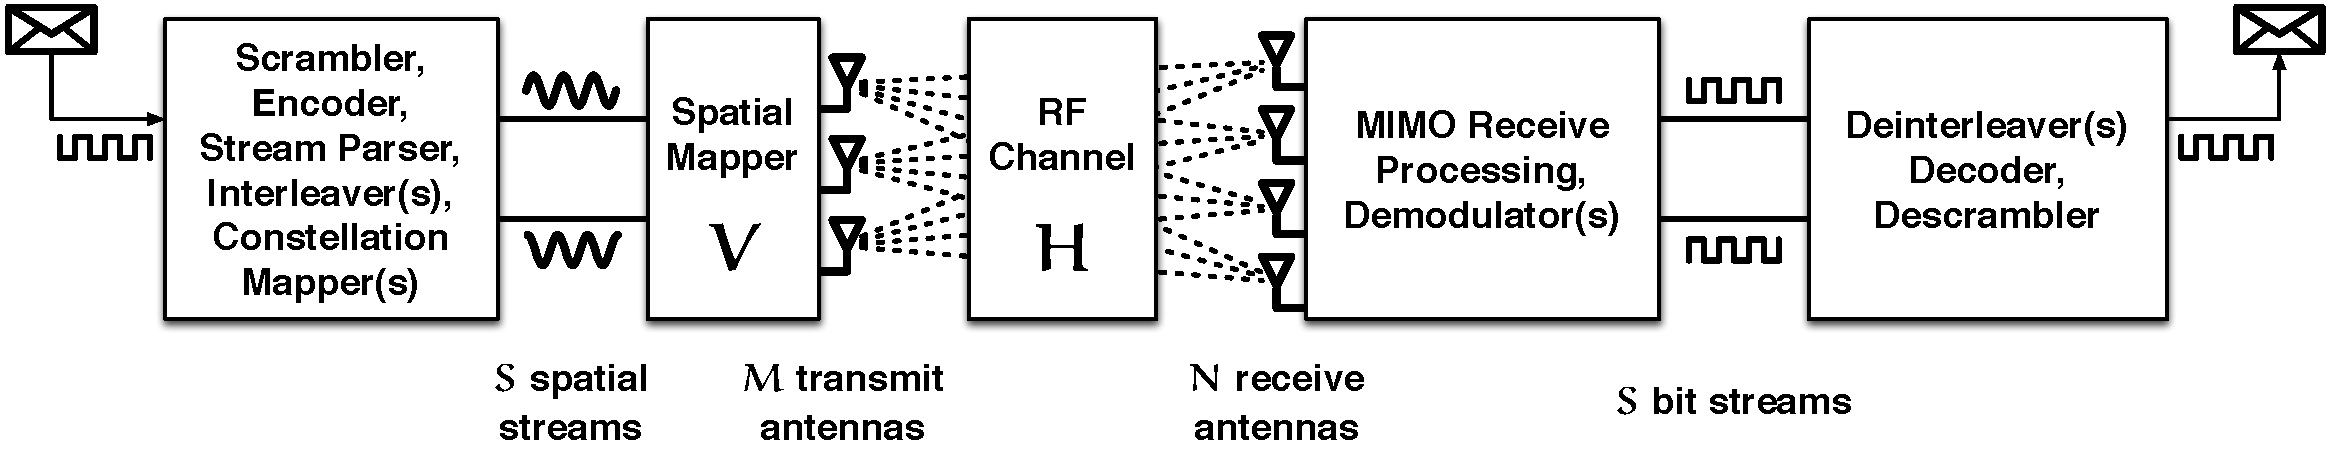
\includegraphics[width=\textwidth]{figures/11n_link_simplified_bigger_fonts.pdf}
\caption[An 802.11n link]{\label{fig:11n_link_simplified}A detailed view of a MIMO-OFDM link in the context of 802.11n.}
\end{figure}

\section{Overview of a MIMO-OFDM Link}
\label{sec:11n_overview}

I begin with a detailed description of a MIMO-OFDM link in the context of 802.11n in order to explain the configuration space and implementation-specific choices that my model my model must support (\figref{fig:11n_link_simplified}). The first block shows standard transmitter processing that generates $S$ spatial streams of modulated symbols from the packet. The internals of this block scramble the original packet to randomize the bits, add error correction, then split the coded bits across the $S$ spatial streams and interleave them between the OFDM subcarriers. These steps spread bits that are coded together across frequency- and spatially-diverse subchannels, after which the transmitter modulates the spread bits into the $S$ streams.

The second block is the \define{spatial mapper} $\mathbf{V}$, which maps the $S$ spatial streams to the $M$ transmit antennas. Different spatial mapping algorithms might map each stream to a single antenna, send a linear combination of each stream to each antenna, or (when $S<M$) use \define{Space-Time Block Codes (STBC)} to take advantage of the extra spatial diversity.

These signals then propagate across the RF channel $\mathbf{H}$ to the $N$ receive antennas. Note that although the figure shows a single RF channel $\mathbf{H}$, the channel can actually be different for every OFDM subcarrier. Consequently, transmitters with the ability to use beamforming can choose for each subcarrier $i$ a different spatial mapping $\mathbf{V}_i$ designed to make the best use of the channel $\mathbf{H}_i$.

After reception, the receiver employs one of many MIMO processing algorithms (i.e., MIMO equalizers) to disentangle the $S$ streams from the $N$ received signals, and demodulates the symbols to recover $S$ (potentially errored) streams of bits. This can be \define{hard demodulation} that simply outputs bits, or \define{soft demodulation} (\cite[\S5.3.1.3]{Sklar},\cite{Jamieson_PPR}) that includes a confidence value for each decoded bit based on the amount of noise in the channel.

In the last block, the receiver deinterleaves and decodes the coded bits, and then descrambles them to undo the transmit processing and recover the original bit stream. At this point, IEEE 802.11n devices typically compute the checksum of the received data and if correct, deliver the packet to the network stack on the host. This completes the description of the most important operations in the sending of a packet from transmitter to receiver in an 802.11n link.

I separated the link into the blocks shown to reflect the considerations that a practical model must handle. The transmitter operation in the first block is completely specified by the IEEE 802.11n standard and the selected rate and channel width. In contrast, the transmitter has a wide choice of spatial mapping matrices to implement unspecified antenna selection, transmit power control, and beamforming algorithms, among others. The receiver can adapt its configuration in response to the channel, for instance by disabling certain antennas and receive chains to save power. To process the received signals there are several MIMO equalizers, demodulation techniques, and error correction decoders that trade off complexity, cost, and performance, and the standard leaves these choices to the implementor. A practical model must be general and flexible to support these many algorithmic and implementation concerns.

%%%%%%%%%%%%%%%%%%%%%%%%%%%%%%%%%%%%%%%%%%%%%%%%%%%%%%%%%%%%%%%%%%%%%%%%%%%%%%%%%%%%%%%%%%
\begin{figure}[ht]
\centering
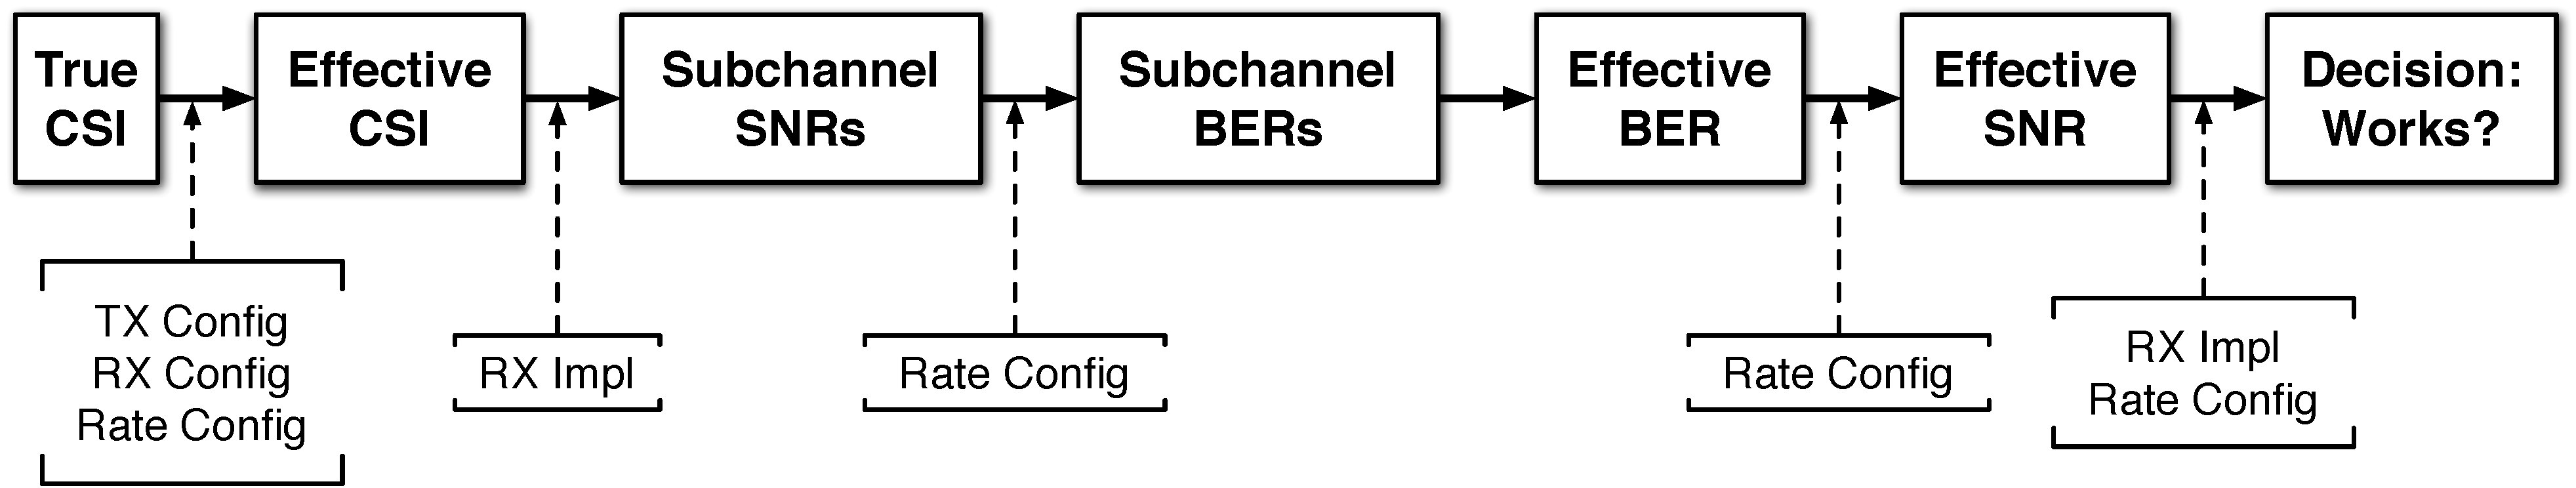
\includegraphics[width=\textwidth]{figures/esnr_model_overview.pdf}
\caption[Model overview]{\label{fig:model_overview}Overview of my Effective SNR-based model for wireless links. The model takes as input a CSI measurement (the ``true CSI'') along with a transmitter configuration, receiver configuration, rate configuration, and some information on the receiver implementation. The output is a single bit that determines whether the link will deliver a packet using the specified rate and device configurations.}
\end{figure}

\section{Effective SNR Model Overview}
\label{sec:model_overview}
\figref{fig:model_overview} gives an overview of my Effective SNR-based model for wireless links, designed to handle the cases described in the previous section. At the left, the primary input to the model is an RF measurement of the ground truth CSI for the wireless link. In the context of MIMO-OFDM technology such as IEEE 802.11n, this is the set of $N$x$M$ matrices $\mathbf{H}_i$, where each matrix describes the MIMO channel between the $M$ transmit and $N$ receive antennas for one OFDM subcarrier.

The other inputs to the model are the configuration of the transmitter and receiver devices, the rate configuration, and some information about the receiver implementation. The final output of the model is a single bit that indicates whether the link will deliver a packet using the specified rate and device configurations. This model can flexibly handle a wide variety of applications: By varying the input transmitter, receiver, and rate configurations, we can solve all the problems described in \chapref{chap:problem}.

In the rest of this chapter, I explain each step of my model. To ease exposition, I start with the core Effective $E_b/N_0$ algorithm from Nanda and Rege~\cite{Nanda_EffectiveSNR}, by which I convert Subchannel SNRs to an Effective SNR, and use this Effective SNR to compute the output decision. I then make the model concrete in the context of IEEE 802.11n by explaining how we can calculate the Subchannel SNRs from the Effective CSI. Next I explain how to compute the Effective CSI, and thus support a variety of applications. Finally, I conclude by discussing how this model can be used in practical scenarios, including which side of the link performs the computation and what information is communicated.

\begin{table}
\centering
\begin{tabular}{cl}
\toprule%
Variable & Meaning\\
\midrule%
$M$ & Number of transmit antennas\\
$N$ & Number of receive antennas\\
$S$ & Number of spatial streams\\
$T$ & Number of OFDM subcarriers (tones) \\
$\mathbf{H}$ & Channel state matrix\\
$\mathbf{V}$ & Spatial mapping matrix\\
$C=ST$ & Number of subchannels \\
$i,j$ & Subchannel indices\\
$\rho$ & Signal-to-noise ratio (SNR) \\
$\beta$ & Bit error rate (BER) \\
$k$ & Number of bits per symbol \\
$\rho_\text{eff}, \beta_\text{eff}$ & Effective SNR or BER\\
$\mathbf{V}_i, \mathbf{H}_i$ & Per-subcarrier spatial mapping or channel state matrix\\
$m$ & Modulation and coding scheme (MCS) index \\
$\tau_m$ & Effective SNR threshold for \mcs{$m$} \\
\bottomrule
\end{tabular}
\caption{\label{tab:notation}Table of notation}
\end{table}

%\begin{table}
%\centering
%\begin{tabular}{cc}
%\toprule%
%\textbf{Function} & \textbf{Computes}\\
%\midrule%
%$\text{BER}_k(\rho)$ & The bit error rate using the 802.11 modulation identified by $k$ at SNR $\rho$\\
%$Q(\cdot)$ & The tail probability (Complementary CDF) of the standard normal function. \\
%\bottomrule
%\end{tabular}
%\caption{\label{tab:functions}Table of functions}
%\end{table}

\begin{table}
\centering
%\footnotesize
\begin{tabular}{ccc}
\toprule
Modulation & Bits/Symbol ($k$) & BER$_k$($\rho$) \\
\midrule BPSK & 1 & $Q\left(\sqrt{2\rho}\right)$ \\
QPSK & 2 & $Q\left(\sqrt{\rho}\right)$\\
16-QAM & 4 & $\frac{3}{4}Q\left(\sqrt{\rho/5}\right)$\\
64-QAM & 6 & $\frac{7}{12}Q\left(\sqrt{\rho/21}\right)$\\
256-QAM$^*$ & 8 & $\frac{15}{32}Q\left(\sqrt{\rho/85}\right)$\\
\bottomrule
\end{tabular}
\caption[Bit error rate as a function of the symbol SNR for OFDM modulations]{\label{tab:ber_snr}Bit error rate as a function of the symbol SNR $\rho$ for narrowband signals and OFDM modulations. $Q$ is the standard normal CCDF. *IEEE 802.11ac will add 256-QAM.}
\end{table}

%%%%%%%%%%%%%%%%%%%%%%%%%%%%%%%%%%%%%%%%%%%%%%%%%%%%%%%%%%%%%%%%%%%%%%%%%%%%%%%%%%%%%%%%%%
\section{Computing Effective SNR from Subchannel SNRs}
At the core of my model is the Effective $E_b/N_0$ algorithm from Nanda and Rege~\cite{Nanda_EffectiveSNR}, which works as follows. Suppose that we are given a set of Subchannel SNRs, indexed such that $\rho_i$ corresponds to the SNR for the $i$th subchannel, $i\in1\dots C$.

The first step is to convert the Subchannel SNRs to Subchannel BERs. In \tabref{tab:ber_snr}, I give the formulas that relate SNR to BER for the modulations used in 802.11. These are adapted from textbook formulas~\cite[\S3.7.1 and \S7.9.3.1]{Sklar} to use the SNR that is measured by wireless NICs instead of the $E_b/N_0$ that is traditionally used in textbooks. Because different modulations have distinct constellations, each modulation has a slightly different error rate function identified as $\text{BER}_k$, where $k$ is the number of bits encoded by one symbol. I use $\text{BER}_k^{-1}$ to denote the inverse mapping from BER to SNR.

Because modern technologies use narrowband subchannels (such as OFDM subcarriers), we can assume that these formulas are accurate with respect to subchannel SNR and BER, unlike the packet-level SNR and BER for the entire link. Then we can compute the Effective BER (denoted $\beta_{\text{eff},k}$)
\begin{equation}
	\label{eq:effective_ber}
%	\tag{Effective BER}
	\beta_{\text{eff},k} = \frac{1}{C} \sum_{i}^{C} \text{BER}_k(\rho_i)
\end{equation}
and Effective SNR ($\rho_{\text{eff},k}$)
\begin{equation}
	\label{eq:effective_snr}
%	\tag{Effective SNR}
	\rho_{\text{eff},k} = \text{BER}_k^{-1}(\beta_{\text{eff},k}).
\end{equation}
%SoftRate estimates BER using internal receiver state~\cite{Vutukuru_SoftRate}. We compute it from channel measurements instead.

Note that the BER mapping and hence Effective SNR are functions of the modulation ($k$). That is, unlike the RSSI, a particular wireless channel will have four different Effective SNR values, one describing performance for each of the modulations. In practice, the interesting regions for the four Effective SNRs do not overlap because at a particular Effective SNR value only one modulation will be near the transition from useless (BER $\approx$0.5) to lossless (BER $\approx$0). When graphs in this paper are presented with an Effective SNR axis, we use all four values, each in the appropriate SNR range.

To compute the output decision bit that indicates whether the link will deliver packets, we simply compare the Effective SNR to an MCS-dependent threshold $\tau$:
\begin{equation}
\label{eq:threshold}
\text{works?}_m = (\rho_{\text{eff},k} > \tau_m).
\end{equation}
Note that the \mcs{$m$} specifies the modulation and hence determines which $k$ to use. The thresholds $\tau_m$ are determined by the \emph{receiver implementation}, but are not link- or device-dependent. We can choose $\tau$ in a variety of ways, the most straightforward of which is via measurements over a wired link as in \figref{fig:snr_prr_attenuator}. As in CHARM~\cite{Judd_CHARM}, this model can support different packet lengths with different SNR thresholds.

\subsection{Effective SNR Example}
To make this description concrete, I present an Effective SNR calculation using this core model for an example SISO 802.11n link in \figref{fig:eff_example}.  The subchannels of this single-antenna link are simply the subcarriers, illustrated by the solid line. There is also one line for the Packet SNR, and then four lines that each represent the Effective SNR for a different modulation. Note that the simpler modulations have lower Effective SNRs, but also perform much better at low rates. \tabref{tab:example_bers} shows the Effective BERs for this link.

\begin{figure}[t]
  \centering
  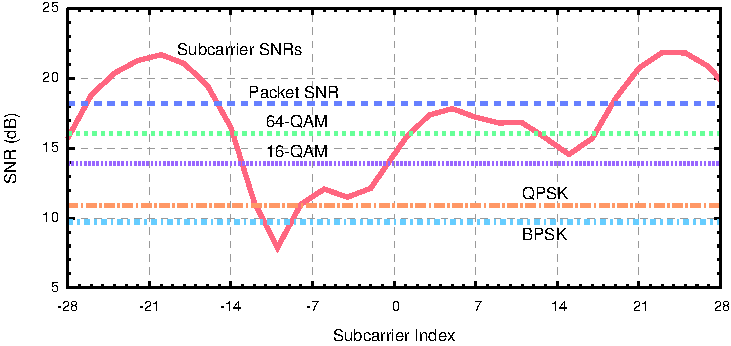
\includegraphics[width=0.9\textwidth]{figures/eff_snr_example.pdf}
  \caption[Packet SNR and Effective SNRs for a sample faded link]{Sample faded link showing the Packet SNR and Effective SNRs for different modulations. BPSK has the lowest Effective SNR, but it needs less energy to decode.}
  \label{fig:eff_example}
\end{figure}

When the Effective SNRs are compared with the pre-determined thresholds for each rate, the model will correctly predict that the best working rate will be 39\Mbps. Note that these Effective SNRs are well below the Packet SNR which is biased towards the stronger subcarriers (note the logarithmic $y$-axis scale). This link does a poor job of harnessing the received power because it is badly faded, so its SNR is a poor predictor of its rate.

\begin{table}[t]
	\centering
	\begin{tabular}{ccc}
	\toprule%
	Modulation & $\rho_\text{eff}$ (dB) & $\text{BER}_\text{eff}$\\
	\midrule%
	BPSK   &  9.7 & $8\times10^{-6}$\\
	QPSK   & 10.9 & $2\times10^{-4}$\\
	16-QAM & 13.9 & $1\%$\\
	64-QAM & 16.1 & $5\%$\\
	\bottomrule
	\end{tabular}
	\caption[Effective SNRs and Effective BERs for the example link in \figref{fig:eff_example}]{\label{tab:example_bers}Effective SNRs and Effective BERs for the example link in \figref{fig:eff_example}.}
\end{table}

\subsection{A Note About Coding}
The astute reader will notice that I did not mention error-correction in the calculations I laid out above. One key decision that makes my model practical is that it is coding-agnostic.

I made this choice because coding interacts with the notion of Effective SNR in a way that is difficult to analyze. One challenge is that the ability to correct bit errors depends on the position of the errors in the data stream. To sidestep this problem, I rely on the interleaving that randomizes the coded bits across subcarriers and spatial streams. Assuming perfect interleaving and robust coding, bit errors in the stream should look no different from bit errors for flat channels (but at a lower SNR). Thus the estimate of the Effective BER in \eqref{eq:effective_ber} will accurately reflect the uncoded error performance of the link. In other words, my model assumes that coding works---but does not care about the details.

Note that this procedure differs from the typical approach of simulation-based analyses~\cite{Kant_FLA, Liu_EESM, Nortel_3g}, which instead map the \emph{uncoded} BER estimate such as I compute to a \emph{coded} BER estimate by means of a log-linear approximation parameterized by the receiver implementation. They then use this coded BER estimate and packet length to directly compute the packet delivery rate of the link. But changing the coding parameters involves changing the internals of the calculation, and with some implementations these parameters can be different for different configurations. (I describe why in the next subsection.) In contrast, all of these effects can be easily expressed, albeit maybe approximately, as (perhaps modulation-dependent) shifts in the Effective SNR thresholds. Thus I believe my method of thresholding the Effective SNR is a better fit because it naturally accommodates these variations.

%Different devices may have different \emph{noise figures}, a measure of how much signal strength is lost in the internal RF circuitry of the NIC\@. They may implement soft Viterbi decoders with more or fewer soft bits for their internal state, or indeed might do hard decoding instead. A receiver could use the optimal Maximum Likelihood MIMO decoder that has exponential complexity for small constellations like BPSK, but revert to the imperfect but more efficient MMSE at higher modulations. All of these can be easily expressed, albeit maybe approximately, as (perhaps modulation-dependent) shifts in the Effective SNR thresholds.

%%%%%%%%%%%%%%%%%%%%%%%%%%%%%%%%%%%%%%%%%%%%%%%%%%%%%%%%%%%%%%%%%%%%%%%%%%%%%%%%%
\section{Modeling the Receiver: Computing Subchannel SNRs from Effective CSI}
\label{sec:model_receiver}
In the last section, I showed how the model of Nanda and Rege~\cite{Nanda_EffectiveSNR} can determine the Effective SNR from a list of Subchannel SNRs. In this section, I explain how to compute the Subchannel SNRs given the Effective Channel State Information of the link.

The \define{Effective CSI} is a $N$x$S$ channel state matrix $\mathbf{H}'$, where each entry describes the gain and phase of each spatial stream as measured at each receive antenna. The columns of the Effective CSI represent \emph{spatial streams}, not \emph{transmit antennas} as in the CSI matrix $\mathbf{H}$. From the point of view of receiver processing the number of transmit antennas used is not relevant, just how the transmitted streams are received after sender-side processing and propagation through the RF channel. I discuss how to compute the Effective CSI in the next section.

Note that the IEEE 802.11 standards do not specify which algorithms the receiver uses to process received signals. However, a small set of techniques are likely chosen in practice: Optimal algorithms or near-optimal techniques that have known, good complexity/optimality tradeoffs. My contact with Intel engineers and marketing documents from other chipset manufacturers confirm that the techniques I present here are the ones used in practice.

Of course, which techniques the receiver might use to process the Effective CSI depends on the dimensionality of the effective channel. In a SISO system, there is little processing to be done, while MIMO systems that use spatial multiplexing and spatial diversity offer lots of options. Hence, I frame my presentation of these techniques around the number of streams and antennas available.

\subsection{SISO links: $S=1,N=1$}
As in the example of \figref{fig:eff_example}, the SNR of a $1$x$1$ channel matrix is simply the power of the single entry in the CSI matrix. There is one Subchannel SNR for each OFDM subcarrier:
\begin{equation}
	\rho_i = \left| \mathbf{H}'_i \right|^2.
\end{equation}

\subsection{SIMO links: $S=1,N>1$}
When there is a single stream and more than one receive antenna, there are two dominant algorithms used. The simpler technique is \define{antenna selection}, in which the antenna with the largest SNR is chosen, and then the SISO algorithm is used on that antenna's signal. The same antenna selection applies to all OFDM subcarriers.
\begin{equation}
	\rho_i = \left| \mathbf{H}'_{i,\hat{a}} \right|^2, \text{where antenna } \hat{a} \text{ has maximal Packet SNR}.
\end{equation}
Some older chipsets, such as the Intel PRO/Wireless 3945~\cite[\S3.5]{ipw3945} and Atheros AR5007~\cite{madwifi_diversity} used antenna selection by default.

The optimal SIMO technique is \define{maximal-ratio combining (MRC)}, which combines the multiple copies of the signal from the different receive antennas. The resulting subcarrier SNR is simply the sum of the SNRs of the individual entries:
\begin{equation}
	\label{eq:mrc}
	\rho_i = \sum_{a=1}^N \left| \mathbf{H}'_{i,a} \right|^2.
\end{equation}
MRC requires more hardware than antenna selection---one receive chain per antenna, instead of one receive chain total. But since spatial multiplexing techniques require multiple receive chains, 802.11n chipsets already have the hardware necessary to perform MRC. The additional computation is minimal, and the resulting gains are large, hence MRC is likely to be used for SIMO links by any 802.11n receiver. Production documentation for Atheros (e.g., the AR6004~\cite{ar6004}) and Realtek (e.g., the RTL8192SU~\cite{rtl8192su}) chipsets and the Intel 802.11n driver source code~\cite{iwlwifi} confirms this assertion.

Devices with more antennas than receive chains can use \define{hybrid selection-combining} algorithms. Such a device might first select the $n < N$ antennas that have the strongest Packet SNRs and then apply MRC to those.

\subsection{MIMO links: $S>1$}
When the transmitter uses spatial multiplexing, i.e.\ $S>1$, the receiver uses a MIMO equalizer to disentangle the streams from its $N\geq S$ receive antennas. For a MIMO link, there are a total of $C=TS$ values for Subchannel SNRs, one per subcarrier (tone) per stream. I denote these $\rho_{i,j}$ where $i$ is an index over tones and $j$ an index over streams. There are several possible techniques that do this; here I discuss the two algorithms most likely to be used in practice.

A \define{Minimum Mean Square Error (MMSE)} MIMO receiver is used by the Intel Wireless Wi-Fi Link 5300 and perhaps other 802.11n devices. For a single stream, MMSE is optimal and equivalent to MRC, and MMSE is near optimal for spatial multiplexing.

The SNR of the $j$th stream after MMSE processing for subcarrier $i$ is given by
\begin{equation}
\centering
\label{eq:mmse_snr}
\rho_{i,j} = \frac{1}{\mathbf{Y}_{jj}}-1, \text{ where }
\mathbf{Y} = \left((\mathbf{H}'_i)^\dagger \mathbf{H}'_i+I_S\right)^{-1}
\end{equation}
for $j \in [1,S]$ and $S$x$S$ identity matrix $I_S$~\cite{Tse}. The operator $(\cdot)^\dagger$ indicates the \define{Hermitian}, or conjugate transpose of the input matrix.

The advantage of MMSE is that it performs well in most cases and has low computational cost, roughly the cost of matrix multiplication and inversion. An alternative is the \emph{Maximum Likelihood (ML)} decoder, but this has added complexity that scales with the size of the constellation, i.e., is exponential in the number of bits per symbol $k$. In the initial 802.11n chipsets, ML decoding was considered too complex to be practical, but this outlook has recently changed. Today, Intel's IWL6300 (successor to the IWL5300 mentioned above) uses ML decoding for the smaller constellations for which it is practical. Atheros uses a ``simplified maximum likelihood detector''~\cite{ar6004,Atheros_11nTechPaper} for all modulations that approximates ML performance but has lower complexity.

The task of estimating the per-stream SNR of the output from a maximum likelihood decoder is non-trivial. Existing estimation techniques, such as the approximation by Redlich et al.~\cite{Redlich_MLSNR}, have the same complexity as the full ML receiver, and are hence impractical for software implementation (though they may be suitable for use if implemented in hardware).

Instead, I observe that maximum likelihood decoding can be approximated as a $\approx$3\dB gain over MMSE for typical MIMO systems~\cite{Kumar_ml_mmse}. Thus, the practical solution I propose for my model is to always compute Effective SNR estimates using MMSE, and instead adapt the decision thresholds $\tau_m$ to reflect the use of ML decoding. This approximation is imprecise---the gains of ML will vary depending on the particular channel---but allows the model to flexibly handle many device implementations (even hybrid MMSE/ML such as in the IWL6300). The error is likely to be small for most channels.

\subsection{Summary}
In this section, I explained how to determine the Subchannel SNRs given Effective CSI matrices for Wi-Fi links. The SISO matrices give the Subchannel SNRs directly, and I assume the use of MRC when modeling SIMO processing; these choices are certain to be accurate because the algorithms are optimal and computationally simple. For MIMO links, the model will always use the MMSE formula given by \eqref{eq:mmse_snr} to compute the Subchannel SNRs, though some receivers may use ML instead. But since the difference between ML and MMSE is often just a few dB, the model will assume MMSE and instead represent the gains from using ML by having lower Effective SNR thresholds. I describe how the sender and receiver might communicate these thresholds later in this chapter. Before doing so, I will next describe the last component of my model needed to make application decisions over a space of configurations.

%%%%%%%%%%%%%%%%%%%%%%%%%%%%%%%%%%%%%%%%%%%%%%%%%%%%%%%%%%%%%%%%%%%%%%%%%%%%%%%%%
\section{Applications: Adapting CSI to Compute Effective CSI}
\label{sec:model_applications}
The last few sections have described how my model can take an Effective CSI and compute the Subchannel SNRs. The final piece is to adapt the CSI $\mathbf{H}$ to determine the Effective CSI $\mathbf{H}'$ that would be measured using a particular configuration, and hence support application decisions. Here, I explain how to perform this step for an illustrative set of these problems.

\heading{Antenna Selection.} There are $N$ rows and $M$ columns in the CSI that each correspond to one transmit or receive antenna. To implement antenna selection, we simply pick the subset of rows and columns that correspond to the desired antennas. Note that this includes both transmit antenna selection (e.g., when $S<M$, pick the best $S$ of the $M$ transmit antennas to send with) or receive antenna selection (e.g., when $N>S$, turn off the least useful of the excess antennas in order to reduce power consumption).

\heading{Channel Width Selection.} In 802.11n, a full 40\MHz CSI measurement comprises 114 matrices $\mathbf{H}_i$. To implement channel width selection, we use only the $\mathbf{H}_i$ covered by the potential channel. For the lower 20\MHz channel, we would use the matrices corresponding to $i \in [1,56]$; for the upper 20\MHz channel we would use the matrices for $i \in [59,114]$. (Subcarriers 57 and 58 are not part of either 20\MHz channel because the 40\MHz channel does not need the same guard band.) This method can also predict performance using 5\MHz or 10\MHz channels as in 802.11j or SampleWidth~\cite{Chandra_SampleWidth}, and could support a potential future version of 802.11 that allows the devices to use non-contiguous tones as in SWIFT~\cite{Rahul_SWIFT}.

\heading{Transmit Power Control.} To emulate the effects of transmit power control, we can simply scale the entries in the matrices $\mathbf{H}_i$. When the transmitter reduces the transmit power uniformly across subcarriers, say by 3\dB, we multiple each matrix by the square root of the power change, in this example by $\sqrt{2}$. To model the effects of asymmetric power control across subchannels, e.g., water filling across streams or subcarriers, we can apply scaling differently to different parts of the channel matrix.

\heading{MCS (Rate) Selection.} For any of the above transmitter and receiver configurations, this process in conjunction with the core algorithms described in the last two sections can predict whether a particular MCS will reliably deliver packets. The CSI matrix may need to be slightly modified depending on the MCS, however. For instance, when using multiple streams the total amount of power is generally kept constant, so the Effective CSI must include a division of the transmit power across antennas. Similarly, some chipsets (e.g., IWL5300 and the Atheros-based Ubiquiti SR71-A~\cite{sr71a}) are unable to send at full power when using the highest modulations, because the peak-to-average power ratio (PAPR) is higher than the transmit amplifier(s) can support. For these chipsets, the Effective CSI must be scaled to compensate for the reduced transmit power when predicting the performance of the relevant modulations.

\heading{Spatial Mapping.} Spatial mapping algorithms determine how the different transmit streams are mapped to transmit antennas. These are implemented by the $N$x$S$ matrices $\mathbf{V}_i$, such that the Effective SNR is
\begin{equation}
	\mathbf{H}'_i = \mathbf{H}_i\mathbf{V}_i.
\end{equation}
I discuss the four types of spatial mapping techniques from the simplest to the most general.

\begin{itemize}[leftmargin=0.5cm,parsep=1ex,itemsep=1ex,topsep=1ex]
	\item In \define{direct mapping}, the transmitter maps each spatial stream directly to one of $S$ antennas; excess antennas go unused. After choosing the appropriate rows of $\mathbf{H}$ as described above under transmit antenna selection, the matrix $\mathbf{V}$ is the identity matrix $I_S$. We can combine transmit antenna selection and direct mapping using a $M$x$S$ matrix $\mathbf{V}$ consisting of zeros except for the $S$ entries in different rows and columns that indicate which streams are mapped to which antennas. For $S=2$ and $M=3$, a direct mapping matrix using the first and third antennas would be
	\begin{equation*}
		\tag{Combined $3$x$2$ TX Antenna Selection and Direct Mapping}
		\mathbf{V} = \begin{pmatrix}
		1 & 0\\
		0 & 0\\
		0 & 1
		\end{pmatrix}.
	\end{equation*}
%
	\item In \define{indirect mapping}, the $S$ streams are mapped to $S$ antennas but in such a way as to be spread over multiple antennas. For instance, the IWL5300 uses the following indirect mapping for 3 streams and 20\MHz channels:
	\begin{equation*}
		\tag{IWL5300 $3$x$3$}
		\mathbf{V} = \begin{pmatrix}
		e^{-i2\pi/16} & e^{-2i\pi/(80/33)} & e^{-2i\pi/(80/3)} \\
		e^{-i2\pi/(80/23)} & e^{-2i\pi/(48/13)} & e^{-2i\pi/(240/13)} \\
		e^{-i2\pi/(80/13)} & e^{-2i\pi/(240/37)} & e^{-2i\pi/(48/13)}
		\end{pmatrix}.
	\end{equation*}
	Atheros uses Walsh (also called Hadamard) spreading. The $2$x$2$ mapping is:
	\begin{equation*}
		\tag{Atheros $2$x$2$}
		\mathbf{V} = \begin{pmatrix}
		1 & 1\\
		1 & -1
		\end{pmatrix}.
	\end{equation*}
%
	\item When using \define{spatial expansion}, $S$ spatial streams are mapped to $M > S$ transmit antennas. Here, $\mathbf{V}$ is the product of an expansion matrix and one of the direct or indirect mapping matrices above. I show the case of $S=2$ and $M=3$ using a sample expansion matrix from the 802.11n standard:
	\begin{equation*}
		\tag{$3$x$2$ Spatial Expansion}
		\mathbf{V} = \sqrt{\frac{2}{3}}\begin{pmatrix}
		1 & 0\\
		0 & 1\\
		1 & 0
		\end{pmatrix}\mathbf{V}',
	\end{equation*}
	where $\mathbf{V}'$ is a direct or indirect mapping matrix. The $\sqrt{2/3}$ factor above represents the even spreading of the power from 2 streams across 3 antennas.
%
	\item Finally, \define{beamforming} is a general technique for mapping streams to antennas. Beamforming can be thought of as a synthesis of indirect mapping, spatial expansion (if applicable) and transmit power control. The distinctive feature of beamforming compared with the above is that it is \emph{channel-aware}; in other words, the beamforming matrix is chosen to improve performance based on the known current channel $\mathbf{H}$. This means that beamforming can use different mapping matrices $\mathbf{V}_i$ for each subcarrier, unlike the prior techniques which are applied uniformly across tones. There are a large variety of techniques that use beamforming to improve the channel, but all can be represented in matrix form.
\end{itemize}

\heading{Higher-level Applications.} To implement applications that require the composition of multiple measurements, such as channel selection, path selection, or access point selection, we can repeat the steps above. For instance, two devices that wish to find the operating channel on which their link is fastest need only frequency-hop in unison and take CSI measurements for each frequency. They can then use the model to predict the achievable bitrate of each measured operating channel and select the fastest.

%%%%%%%%%%%%%%%%%%%%%%%%%%%%%%%%%%%%%%%%%%%%%%%%%%%%%%%%%%%%%%%%%%%%%%%%%%%%%%%%%%%%%%%%%%%%%%%%%%%%%%%%%
\section{Protocol Details}
\label{sec:model_protocol}

In this section I make concrete the actual protocols and algorithms by which my Effective SNR model can be used. Decisions about which configuration to choose can be made by either end of the link, and each has its advantages. I begin by presenting an algorithmic overview of my model and the set of information needed to compute it. I then discuss transmit-side and receiver-side procedures for calculating the Effective SNR, including what information needs to be communicated between endpoints, and when that exchange happens, for these approaches to work.

\subsection{Protocol Overview}
%%%%%%%%%%%%%%%%%%%%%%%%%%%%%%%%%%%%%%%%%%%%%%%%
\begin{algorithm}[tp]
\caption{\label{alg:eff_snr_basic}\fcall{Effective SNR Algorithm Skeleton}}
\begin{algorithmic}[1]
\STATE Define an application by a set of configurations $\mathcal{C}$ and a metric $\mathcal{M}$
\STATE Measure the CSI $\mathbf{H}$, covering the subchannels used in all configurations
\FOR {configuration $c_i \in \mathcal{C}$}
\STATE Use the Effective SNR model and $\mathbf{H}$ to determine whether $c_i$ works \COMMENT{Note that $c_i$ specifies a choice of rate, sender configuration (including channel), and receiver configuration.\hspace{-1in}}
\IF {configuration $c_i$ works}
\STATE set metric $m_i$ to $\mathcal{M}(c_i)$
\ELSE
\STATE set metric $m_i$ to 0 (or $\infty$ as appropriate)
\ENDIF
\ENDFOR
\RETURN the configuration $c_i$ with the best metric $m_i$
\end{algorithmic}
\end{algorithm}
%%%%%%%%%%%%%%%%%%%%%%%%%%%%%%%%%%%%%%%%%%%%%%%%
I present the skeleton of a procedure to use my Effective SNR model as \algref{alg:eff_snr_basic}. We can define an application as a set of configurations under consideration ($\mathcal{C}$) and some metric ($\mathcal{M}$) that enables us to choose between configurations. For the example case of rate selection, we might define $\mathcal{C}$ to be all 24 SIMO, MIMO2, and MIMO3 transmit configurations with the receiver fixed to use all 3 antennas, and the metric $\mathcal{M}$ to be the raw bitrate (6.5\Mbps--195\Mbps) of each configuration. \algref{alg:eff_snr_basic} will use my Effective SNR procedure on a measured 3x3 channel matrix $\mathbf{H}$ to evaluate which of these 24 configurations will reliably deliver packets, and then return the fastest working configuration.

In order to actually run this procedure, three pieces of information are necessary in practice:
\begin{enumerate}[parsep=1ex,itemsep=1ex,topsep=1ex]
	\item Up-to-date CSI measurements including all relevant subchannels.
	\item The receiver's MCS-specific Effective SNR thresholds.
	\item Knowledge of how to compute the Effective CSI $\mathbf{H}'$ from the CSI $\mathbf{H}$.
\end{enumerate}
A challenge is that this information is spread across the transmitter and receiver. In particular, CSI measurements are naturally measured at the receiver in the course of receiving 802.11n packets, and I envision that the receiver's Effective SNR thresholds will be programmed in at the factory since they are fixed and independent of channel conditions. At the same time, computing the Effective CSI requires knowledge of transmitter behavior, including spatial mapping matrices as well as any implementation-specific oddities. The latter can be quite broadly defined, such as Intel's reduction of transmit power by up to 5\dB for the highest 64-QAM single-stream encodings to compensate for amplifier non-linearities. Finally, which endpoint applies the result of the computation depends on the application in mind. Often the adjustment will be at the transmitter side, such as choice of rate, but some applications, such as receive antenna selection, are applied at the receiver.

In the next few subsections, I first discuss how CSI is obtained, as this is the main run-time measurement needed to run this algorithm. I then describe the transmitter- and receiver-side ways to implement \algref{alg:eff_snr_basic} and the tradeoffs of the various approaches. The primary tradeoff is between the amount of data shared (because the party performing the calculation needs up-to-date CSI) and protocol complexity.

\subsection{CSI Collection}
\label{sec:csi_collection}
As with RSSI, receivers gather channel state information automatically while receiving a packet; the OFDM and MIMO equalizers described in \secref{sec:model_receiver} fundamentally rely on CSI to decode the received signal. This \emph{passive collection} of CSI via overheard transmissions suffices for most applications, such as rate selection. When a more comprehensive CSI measurement is needed, the transmitter can send a sounding packet~\cite[\S20.3.13.1]{80211n} at a wider bandwidth or using more streams to probe the extra dimensions. For the special case of additional spatial streams, 802.11n includes a mechanism to send a modified packet with \define{extension spatial streams}~\cite[\S20.3.9.4.6]{80211n} such that the receiver can measure the full channel during the preamble but that does not change the rate or number of streams used for the data portion.

\subsection{Transmitter-side Computation}
The transmitter seems to be a natural place to perform these computations, as most configuration points are determined by transmitter configurations. To do so, it needs an up-to-date CSI measurement as well as the receiver's MCS thresholds. The latter is easy: Since the thresholds are fixed for a particular model of NIC, they can be shared by the receiver once, e.g., during association.

The transmitter can obtain CSI via feedback or estimated implicitly from the reverse path. When the receiver feeds CSI back to the transmitter, this process adds latency and reduces airtime efficiency. 802.11n includes mechanisms to limit these effects via rapid feedback protocols~\cite[\S9.19.2]{80211n} and compressed CSI feedback formats~\cite[\S20.3.12.2.5]{80211n}. Additionally, my measurements taken in conjunction with experimenters at Intel show that in slow-fading channels, such as static nodes with indoor mobility, CSI estimates are valid for a few hundred milliseconds~\cite{Perahia_Doppler} and this may require less frequent feedback.

Alternatively, the transmitter can attempt to estimate the CSI implicitly when receiving packets, such as ACKs, sent by the receiver. This is the standard approach taken in Packet SNR-based schemes such as CHARM~\cite{Judd_CHARM} proposed for 802.11a. For 802.11n, this approach mandates that the receiver inform the transmitter of its spatial mapping matrices, and use all its antennas to send these packets. Some receivers, such as the Intel IWL5100, have more receive antennas than transmit chains, and cannot send on all antennas. For these devices, implicit feedback would simply not work. The other receivers would need to alternate transmit antennas while the transmitter used CSI Sampling and Fusion~\cite{Crepaldi_CSI_SF} to build up a complete CSI. The use of implicit feedback also requires devices to use the 802.11n calibration process to compensate for hardware differences in the measured transmit and receive chains and those that will be used when the two devices swap roles.

Finally, the implicit feedback approach induces all the problems of receiver-side computation with few of the benefits, and I don't find it to be practical. Instead, I recommend that the transmitter obtain CSI feedback explicitly when making an Effective SNR decision.

\subsection{Receiver-side Computation}
The other approach is for the receiver to perform the computations and make the application decisions, feeding them back to the transmitter when necessary. This obviates sending CSI and speeds up the protocols, but instead requires that the receiver understand the transmitter's behavior.

Today, the transmitter shares some of these details, such as number of transmit antennas and whether it supports optional 802.11n features, with the receiver during association. But the standard does not include a method by which a transmitter can share its spatial mapping matrices, and it's not immediately clear that this would sufficiently capture all implementation artifacts such as those described above.

The other drawback to this approach is that it complicates receiver algorithms. For instance, if the transmitter is an access point and the client a cell phone, the former device is likely to have much more sophisticated silicon. We have seen this today as many 802.11 manufacturers have targeted systems with asymmetric capabilities such that the access point shoulders all the computation load, reducing the complexity and hence cost of the client which need only support basic functionality. The receiver-side approach requires that the receiver shoulder the computational load of running the model and making decisions; in contrast for the transmitter-side approach it must only support CSI feedback.

Still, I believe that the receiver-side approach is fundamentally the best. It has the primary advantage of putting the computation near the data, so that rather than feeding back the full CSI measurement to the transmitter it need only send the application decision over the wire. This is similar to the approach taken by RBAR~\cite{Holland_RBAR}, and support for this has been added to 802.11 with the new 802.11n Link Adaptation Control field~\cite[\S7.1.3.5a]{80211n} that can embed feedback in packet headers, including ACKs, to directly request a particular MCS, select transmit antennas, or request a particular beamforming (or other spatial mapping) matrix.

To make the receiver-side algorithm work best, I suggest a simple new contract be added to 802.11n as a standard requirement. Since today transmitters may use fundamentally different spatial mapping matrices for different numbers of streams, it is hard to convert compute the Effective CSI for a different number of streams. Indeed, the Intel IWL5300 uses spatial mapping matrices such that the 2-stream CSI bears no obvious relation to the 3-stream CSI without knowledge of the possible mappings, and uses different matrices for 20\MHz and 40\MHz channels.  I propose that transmitter spatial mapping matrices be restricted such that when a receiver subsets a large (e.g., MIMO3) CSI measurement to simulate a smaller (e.g., MIMO2) configuration, the result indeed corresponds to the channel that would be measured if the transmitter used that mode. The alternative---sharing the full extent of these mappings---is hard to fit into a clean protocol, so I think this new contract would best resolve the situation without greatly compromising transmitter performance or flexibility.

\subsection{Summary}
In this section, I discussed practical details of implementing my Effective SNR-based decision procedure. When comparing the transmitter-side and receiver-side options for implementing this functionality, I concluded that receiver-side computation likely represents the best tradeoff, because it has the benefit of low overhead without compromising on flexibility, accuracy, or agility.

In certain situations, such as when selecting beamforming matrices, the decision may be best made at the transmitter, which better understands the limitations of its own hardware. And for multiple links to coordinate, CSI measurements may need to be shared in a local neighborhood. One example of a system that does this lightweight local sharing in order to achieve better spatial reuse is IAC~\cite{Gollakota_IAC}.

%%%%%%%%%%%%%%%%%%%%%%%%%%%%%%%%%%%%%%%%%%%%%%%%%%%%%%%%%%%%%%%%%%%%%%%%%%%%%%%%%%%%%%%%%%%%%%%%%%%%%%%%%
\section{Comparison to Other Techniques}
I conclude this chapter by comparing my Effective SNR to other techniques that use physical layer or other low-level information to predict the performance of a wireless link. I compare algorithms along two axes: (1) their accuracy and ability to flexible handle many configuration problems, and (2) their fundamental properties in terms of overheads and responsiveness.

\begin{table}[ht]
\centering
\begin{tabular}{ccccccc}
\toprule
\multirow{2}{*}{Algorithm} & \multirow{2}{*}{802.11a/b/g} & 802.11n & Antenna & \multirow{2}{*}{TX Power} & Channel & \multirow{2}{*}{Real NICs} \\
& & (MIMO) & Selection & & Width \\
\midrule
Packet SNR & ? & & & & & \checkmark\\
SoftRate~\cite{Vutukuru_SoftRate} & \checkmark \\
AccuRate~\cite{Sen_AccuRate} & \checkmark & & & \checkmark & \checkmark \\
EEC~\cite{Chen_EEC} & \checkmark & & & & & \checkmark \\
Effective SNR & \checkmark & \checkmark & \checkmark & \checkmark & \checkmark & \checkmark\\
\bottomrule
\end{tabular}
\caption[Comparison of link error rate prediction algorithm accuracy]{\label{tab:algorithm_comparison}A comparison of Effective SNR to other recent algorithms that purport to predict the performance of a wireless link. Effective SNR can predict packet delivery in the largest space because it looks at the raw channel response, whereas the other techniques mostly apply only to single-stream links with fixed antennas and transmit power.}
\end{table}


\subsection{Accuracy}
\tabref{tab:algorithm_comparison} summarizes the comparison between Effective SNR and other recent algorithms that aim to predict the performance of a wireless link. The results show that Effective SNR can handle a much broader problem space because it looks at the raw channel details, while other algorithms primarily apply only to single-stream links with fixed antennas and transmit power.

As I presented in the previous section, Packet SNR based on RSSI is available in today's devices, but does not accurately predict performance for 802.11a/g due to its inability to capture frequency-selective fading; the use of MIMO in 802.11n only exacerbates this deficiency.

SoftRate~\cite{Vutukuru_SoftRate} and EEC~\cite{Chen_EEC} both use information from the error correction hardware to accurately measure the Effective BER of the \emph{current} configuration and work well for rate selection using adjacent 802.11a/b/g rates, but cannot predict the performance using other configurations.

AccuRate~\cite{Sen_AccuRate} uses the measured receive error vectors as input to a full channel simulator; like my model this procedure can estimate the Effective BER of all modulations in the current configuration. However, these computations are computationally expensive and do not work across other applications. The exception is transmit power control; I believe this can be simulated by scaling the error vectors although this approach was not explored by the authors.

In contrast, Effective SNR extends to a significantly larger class of applications than the other techniques because its computations are aware of the low-level physical-layer effects of the RF channel, including frequency- and spatially-selective fading. My model is broadly compatible with 802.11n and requires no hardware changes.

\begin{table}[ht]
\centering
\begin{tabular}{ccccc}
\toprule
\multirow{2}{*}{Algorithm} & \multirow{2}{*}{Measurement} & Communication & \multirow{2}{*}{Compute}  & Response  \\
& & Overhead &  & Time\\
\midrule
Probe-based & Multiple packet loss rate & None & Low & High \\
Packet SNR & Preamble & Low & None & High \\
SoftRate~\cite{Vutukuru_SoftRate} & A few full symbols & Low & Low & Low \\
AccuRate~\cite{Sen_AccuRate} & Preamble & Low & High & Low \\
EEC~\cite{Chen_EEC} & Full packet & Low & Medium & Low \\
\multirow{2}{*}{Effective SNR} & \multirow{2}{*}{Preamble} & Low (RX) & \multirow{2}{*}{Low} & \multirow{2}{*}{Low}\\
& & Medium (TX)\\
\bottomrule
\end{tabular}
\caption[Comparison of prediction algorithm overheads and response times]{\label{tab:algorithm_properties}Comparing overheads and response times of Effective SNR and other algorithms. In addition to being more flexible and accurate than the other algorithms (\tabref{tab:algorithm_comparison}), Effective SNR has low measurement and communication overheads, low computational cost, and low response time that match the best aspects of the other algorithms.}
\end{table}

\subsection{Overheads and Response Time}
\tabref{tab:algorithm_properties} summarizes my qualitative comparison of these algorithms in terms of their practical overheads and the achievable response times.

Packet SNR-based algorithms, AccuRate, and Effective SNR all require only a packet preamble to record their measurements. SoftRate, which uses the output of the error correction blocks to estimate Effective BER requires a packet that contains at least a few MIMO-OFDM symbols that fully utilize the available subchannels. EEC requires slightly more bits to accurate estimate the BER (around a full packet), and the standard probe-based approaches today require multiple full-length packet probes to estimate the loss rate of a particular configuration.

None of the schemes have much communication overhead, feeding back only application decisions or concise metrics such as SNR or BER estimates. When using Effective SNR to make decisions that require transmit-side computation (which other algorithms cannot handle at all) Effective SNR must feed CSI back to the transmitter, though the feedback can be compressed and may only need to be sent periodically.

In terms of computation, Packet SNR and SoftRate require none, either directly feeding back the hardware's estimate to the other side of the link or performing a simple local threshold test. Today's probe-based algorithms require a small amount of computation to update loss rate estimates. Among the rest, EEC's custom codes require a medium amount (about 250\us) of computation~\cite{Chen_EEC}. AccuRate has such a large overhead as to make it impractical, because it requires a full wireless channel simulator of a full-length packet in order to compute its output. In contrast, I will show in the next chapter that the Effective SNR computations for rate selection among 24 MCS combinations can be computed in under 4\us, around the time for a single MIMO-OFDM symbol.

Finally, I compare the algorithms on the basis of their responsiveness. The algorithms that are accurate---SoftRate, AccuRate, EEC, and Effective SNR---are respond quickly to changing channels, for those problems that they can handle and assuming that computations finish in time. In contrast, because probe-based algorithms must search a large space and Packet SNR-based algorithms require online training of SNR thresholds, they cannot respond in an agile way in mobile environments.

\subsection{Summary}
In conclusion, the comparisons in this section show that Effective SNR can handle a much larger problem space than comparable algorithms, because my model is able to capture the underlying RF details of the MIMO-OFDM channel, rather than high-level observations of the channel, packet delivery, or error rates. And the comparison along practical grounds in terms of overheads and response time showed that Effective SNR's overheads and response times match the best of the other algorithms, or induce small additional communication cost to support great additional power.

\section{Summary}
This section has presented my Effective SNR model and how to use it in full detail. I concluded with a comparison of my model to other techniques with similar goals, and showed that Effective SNR matches the best properties while providing significantly more power.

Of course, though I have argued that it is great in principle, I have not yet shown that my Effective SNR model is accurate. In order to understand whether this is the case, I built a prototype implementation of my model using a commercial Intel NIC. In the next chapter I describe that implementation, which I use in the rest of this thesis to demonstrate that my Effective SNR model indeed works well and supports a wide space of applications.


%%%%%%%%%%%%%%%%%%%%%%%%%%%%%%%%%%
\ifx\mainfile\undefined
%
% ==========   Bibliography   ==========
%
%\nocite{*}   % include everything in the uwthesis.bib file
\bibliographystyle{plain}
\bibliography{dhalperi_thesis}

\end{document}
\fi
